\subsection{Period $T$ as a function of $B$}

Grebogi and coworkers \cite{Grebogi1988} have studied how the period $T$ is related with the precision.
There they saw that the period $T$ scales with roundoff $\epsilon$ as $T\sim\epsilon^{-d/2}$ where $d$ is the correlation dimension of the chaotic attractor.

Nagaraj et als. \cite{Nagaraj2008} studied the case of switching between two maps.
They saw that the period $T$ of the compound map obtained by switching between two chaotic maps is higher than the period of each map and they found that a random switching improves the results.
Here we have considered sequential switching to avoid the use of another random variable, because it can include its own statistical properties in the time series.

Fig. \ref{fig:period} shows  $T \times B$ in semi logarithmic scale.
The experimental averaged points can be fitted by a straight line expressed as $log_{2}T=m B + b$ where $m$ is the slope and $b$ is the $y$-intercept.
Results for all considered maps are summarized in Table \ref{tabla:periodos}.

\begin{figure}
\centering	
	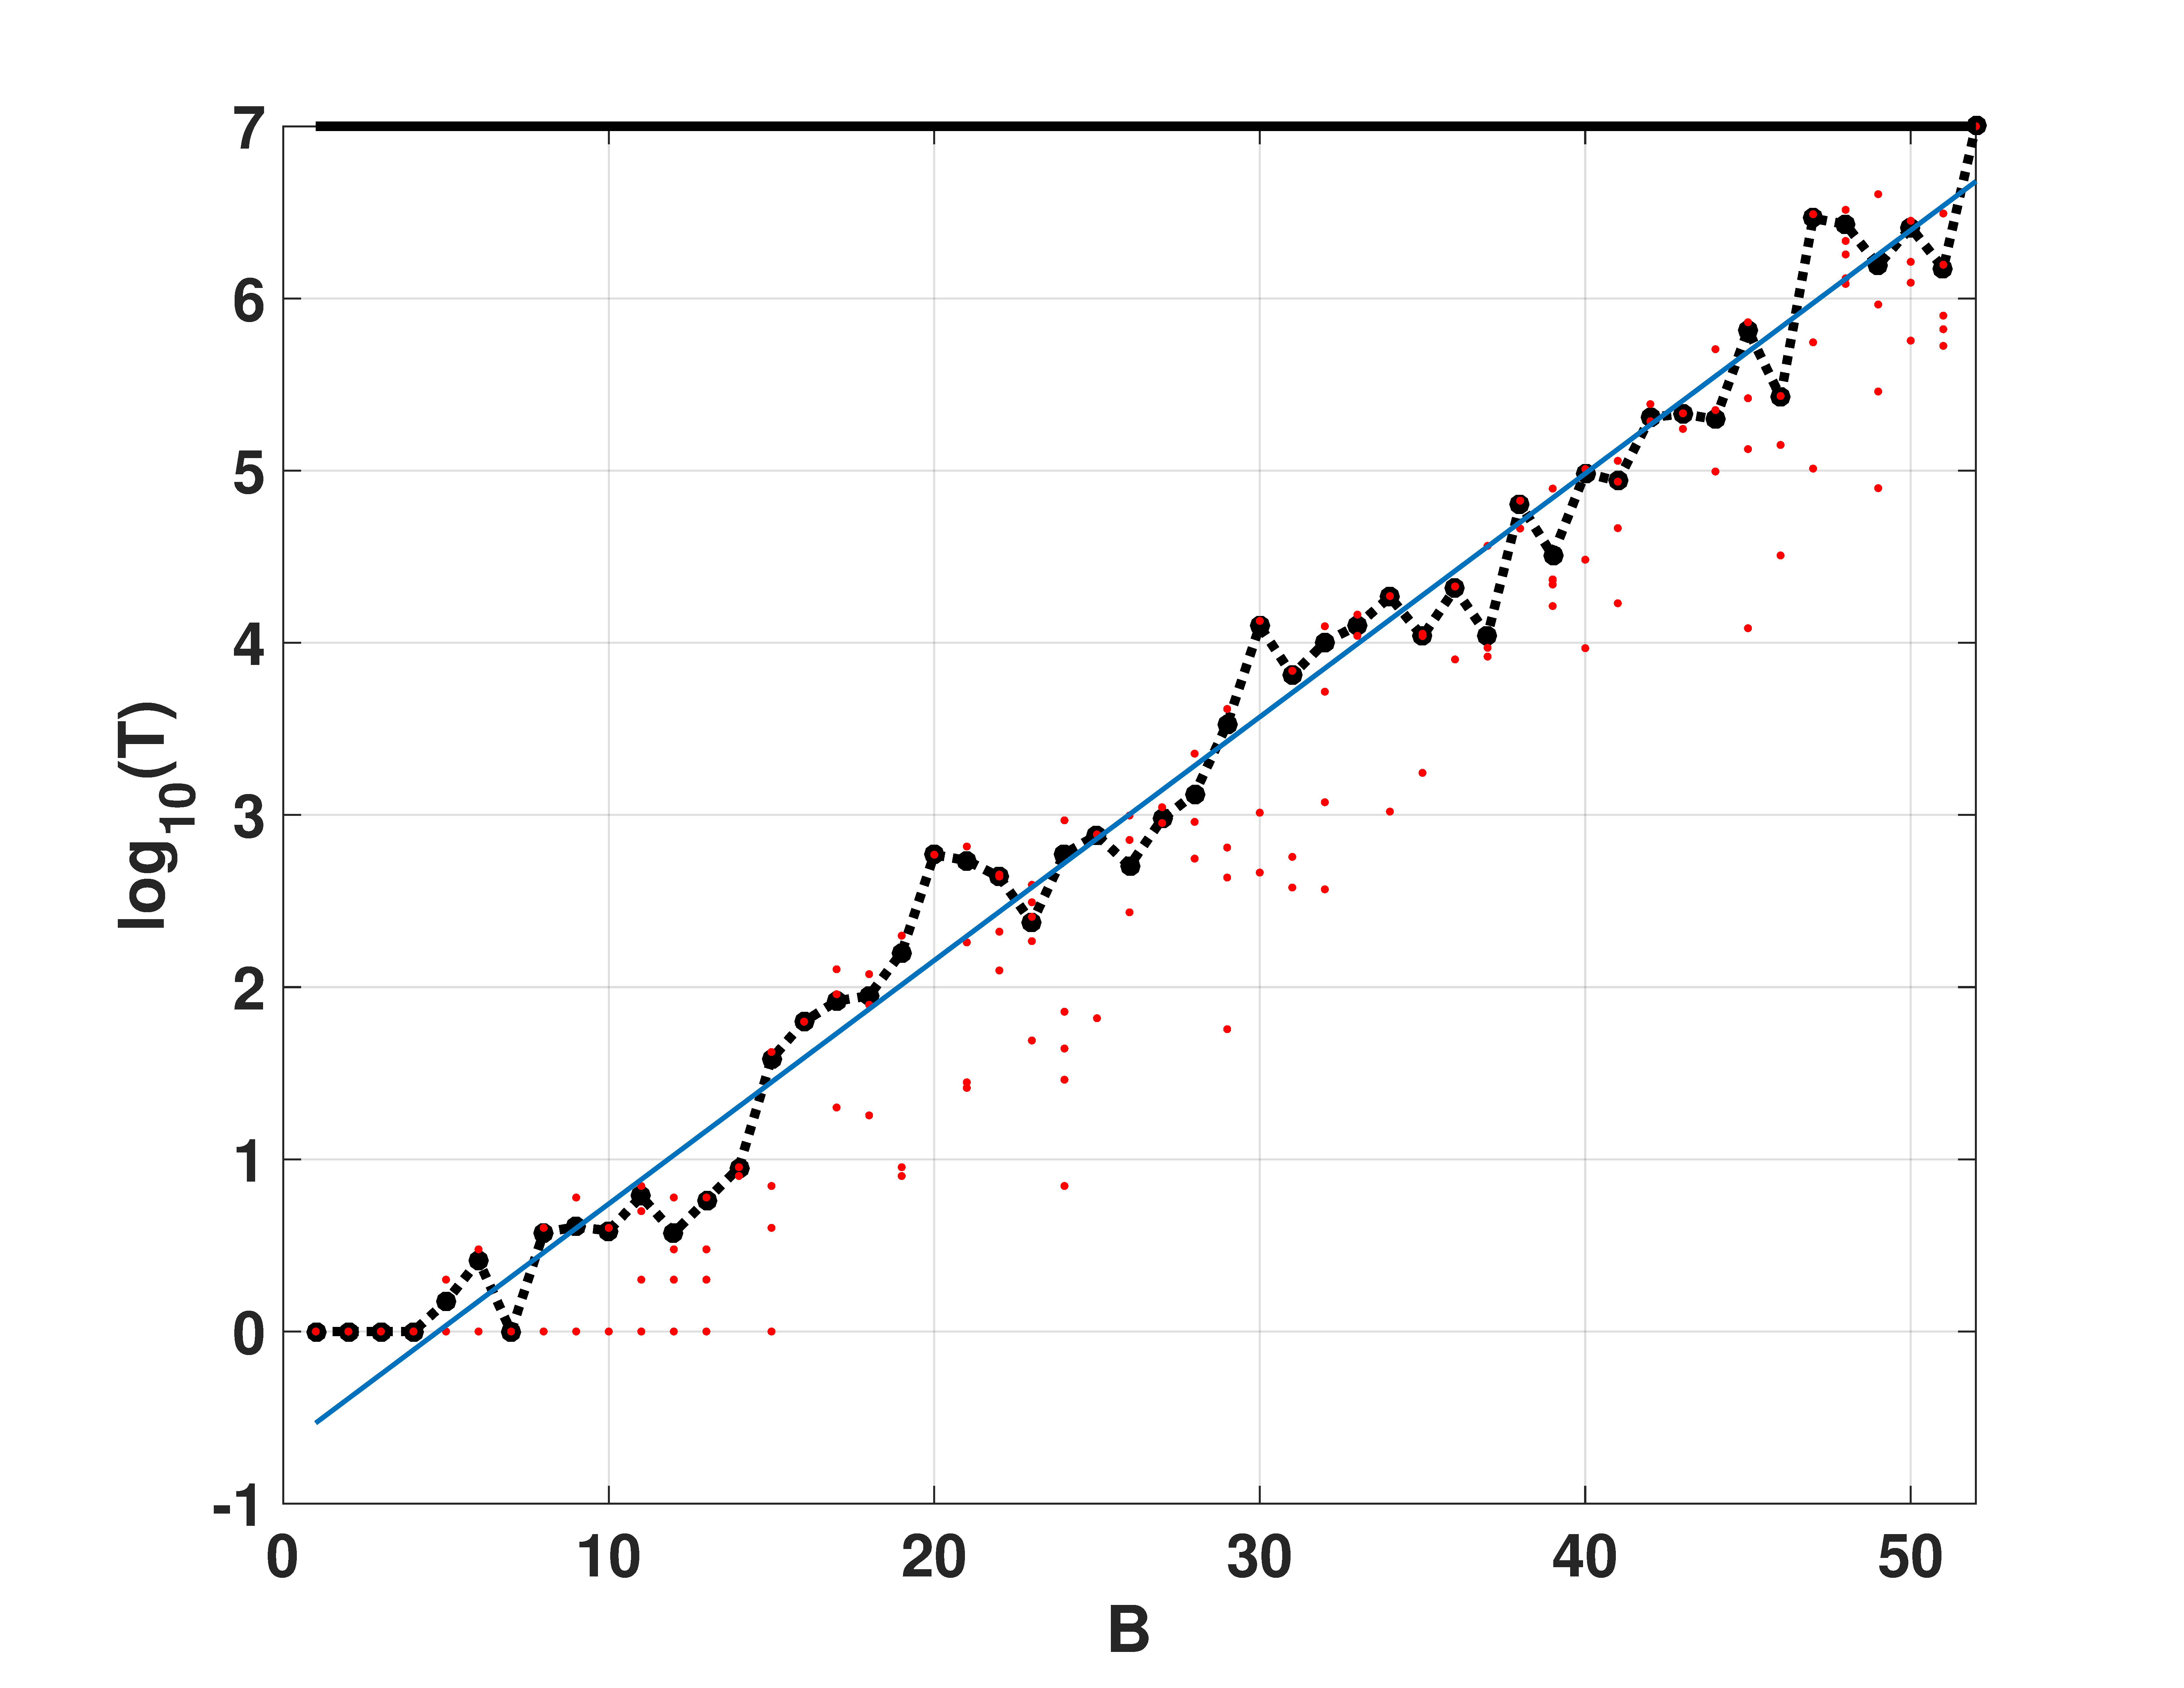
\includegraphics[width=.49\textwidth]{Period_Log}
	\caption{Period as function of precision in binary digits} \label{fig:period}
\end{figure}

\begin{table}
\centering	
	\caption{Period $T$ as a function of $B$ for the maps considered}
	\vspace{1em}
	\begin{tabular}{lll}
		\hline\noalign{\smallskip}
		map & m & b  \\
		\noalign{\smallskip}\hline\noalign{\smallskip}
		TENT&0 & 0 \\
		LOG &0.139 & -0.6188 \\
		SWITCH &0.1462 & -0.5115 \\
		EVEN &0.1447 & -0.7783 \\
		ODD &0.1444 & -0.7683 \\
		\noalign{\smallskip}\hline
	\end{tabular}
	\label{tabla:periodos}	
\end{table}

Results are compatible for those obtained in \cite{Nagaraj2008}.
Switching between maps increases the period $T$ but skipping procedure decreases by almost half.